% Options for packages loaded elsewhere
\PassOptionsToPackage{unicode}{hyperref}
\PassOptionsToPackage{hyphens}{url}
%
\documentclass[
  english,
  man,floatsintext]{apa7}
\usepackage{amsmath,amssymb}
\usepackage{lmodern}
\usepackage{iftex}
\ifPDFTeX
  \usepackage[T1]{fontenc}
  \usepackage[utf8]{inputenc}
  \usepackage{textcomp} % provide euro and other symbols
\else % if luatex or xetex
  \usepackage{unicode-math}
  \defaultfontfeatures{Scale=MatchLowercase}
  \defaultfontfeatures[\rmfamily]{Ligatures=TeX,Scale=1}
\fi
% Use upquote if available, for straight quotes in verbatim environments
\IfFileExists{upquote.sty}{\usepackage{upquote}}{}
\IfFileExists{microtype.sty}{% use microtype if available
  \usepackage[]{microtype}
  \UseMicrotypeSet[protrusion]{basicmath} % disable protrusion for tt fonts
}{}
\makeatletter
\@ifundefined{KOMAClassName}{% if non-KOMA class
  \IfFileExists{parskip.sty}{%
    \usepackage{parskip}
  }{% else
    \setlength{\parindent}{0pt}
    \setlength{\parskip}{6pt plus 2pt minus 1pt}}
}{% if KOMA class
  \KOMAoptions{parskip=half}}
\makeatother
\usepackage{xcolor}
\IfFileExists{xurl.sty}{\usepackage{xurl}}{} % add URL line breaks if available
\IfFileExists{bookmark.sty}{\usepackage{bookmark}}{\usepackage{hyperref}}
\hypersetup{
  pdftitle={The role of cognateness in non-native spoken word recognition},
  pdfauthor={Gonzalo Garcia-Castro1, Serene Siow2, Nuria Sebastian-Galles1, \& Kim Plunkett2},
  pdflang={en-EN},
  pdfkeywords={cognate, word recognition, translation, non-native, spoken word recognition, bayesian},
  hidelinks,
  pdfcreator={LaTeX via pandoc}}
\urlstyle{same} % disable monospaced font for URLs
\usepackage{graphicx}
\makeatletter
\def\maxwidth{\ifdim\Gin@nat@width>\linewidth\linewidth\else\Gin@nat@width\fi}
\def\maxheight{\ifdim\Gin@nat@height>\textheight\textheight\else\Gin@nat@height\fi}
\makeatother
% Scale images if necessary, so that they will not overflow the page
% margins by default, and it is still possible to overwrite the defaults
% using explicit options in \includegraphics[width, height, ...]{}
\setkeys{Gin}{width=\maxwidth,height=\maxheight,keepaspectratio}
% Set default figure placement to htbp
\makeatletter
\def\fps@figure{htbp}
\makeatother
\setlength{\emergencystretch}{3em} % prevent overfull lines
\providecommand{\tightlist}{%
  \setlength{\itemsep}{0pt}\setlength{\parskip}{0pt}}
\setcounter{secnumdepth}{5}
% Make \paragraph and \subparagraph free-standing
\ifx\paragraph\undefined\else
  \let\oldparagraph\paragraph
  \renewcommand{\paragraph}[1]{\oldparagraph{#1}\mbox{}}
\fi
\ifx\subparagraph\undefined\else
  \let\oldsubparagraph\subparagraph
  \renewcommand{\subparagraph}[1]{\oldsubparagraph{#1}\mbox{}}
\fi
% Manuscript styling
\usepackage{upgreek}
\captionsetup{font=singlespacing,justification=justified}

% Table formatting
\usepackage{longtable}
\usepackage{lscape}
% \usepackage[counterclockwise]{rotating}   % Landscape page setup for large tables
\usepackage{multirow}		% Table styling
\usepackage{tabularx}		% Control Column width
\usepackage[flushleft]{threeparttable}	% Allows for three part tables with a specified notes section
\usepackage{threeparttablex}            % Lets threeparttable work with longtable

% Create new environments so endfloat can handle them
% \newenvironment{ltable}
%   {\begin{landscape}\centering\begin{threeparttable}}
%   {\end{threeparttable}\end{landscape}}
\newenvironment{lltable}{\begin{landscape}\centering\begin{ThreePartTable}}{\end{ThreePartTable}\end{landscape}}

% Enables adjusting longtable caption width to table width
% Solution found at http://golatex.de/longtable-mit-caption-so-breit-wie-die-tabelle-t15767.html
\makeatletter
\newcommand\LastLTentrywidth{1em}
\newlength\longtablewidth
\setlength{\longtablewidth}{1in}
\newcommand{\getlongtablewidth}{\begingroup \ifcsname LT@\roman{LT@tables}\endcsname \global\longtablewidth=0pt \renewcommand{\LT@entry}[2]{\global\advance\longtablewidth by ##2\relax\gdef\LastLTentrywidth{##2}}\@nameuse{LT@\roman{LT@tables}} \fi \endgroup}

% \setlength{\parindent}{0.5in}
% \setlength{\parskip}{0pt plus 0pt minus 0pt}

% \usepackage{etoolbox}
\makeatletter
\patchcmd{\HyOrg@maketitle}
  {\section{\normalfont\normalsize\abstractname}}
  {\section*{\normalfont\normalsize\abstractname}}
  {}{\typeout{Failed to patch abstract.}}
\patchcmd{\HyOrg@maketitle}
  {\section{\protect\normalfont{\@title}}}
  {\section*{\protect\normalfont{\@title}}}
  {}{\typeout{Failed to patch title.}}
\makeatother
\shorttitle{Cognateness and non-native word recognition}
\keywords{cognate, word recognition, translation, non-native, spoken word recognition, bayesian\newline\indent Word count: 4553}
\usepackage{lineno}

\linenumbers
\usepackage{csquotes}
\ifXeTeX
  % Load polyglossia as late as possible: uses bidi with RTL langages (e.g. Hebrew, Arabic)
  \usepackage{polyglossia}
  \setmainlanguage[]{english}
\else
  \usepackage[main=english]{babel}
% get rid of language-specific shorthands (see #6817):
\let\LanguageShortHands\languageshorthands
\def\languageshorthands#1{}
\fi
\ifLuaTeX
  \usepackage{selnolig}  % disable illegal ligatures
\fi
\newlength{\cslhangindent}
\setlength{\cslhangindent}{1.5em}
\newlength{\csllabelwidth}
\setlength{\csllabelwidth}{3em}
\newenvironment{CSLReferences}[2] % #1 hanging-ident, #2 entry spacing
 {% don't indent paragraphs
  \setlength{\parindent}{0pt}
  % turn on hanging indent if param 1 is 1
  \ifodd #1 \everypar{\setlength{\hangindent}{\cslhangindent}}\ignorespaces\fi
  % set entry spacing
  \ifnum #2 > 0
  \setlength{\parskip}{#2\baselineskip}
  \fi
 }%
 {}
\usepackage{calc}
\newcommand{\CSLBlock}[1]{#1\hfill\break}
\newcommand{\CSLLeftMargin}[1]{\parbox[t]{\csllabelwidth}{#1}}
\newcommand{\CSLRightInline}[1]{\parbox[t]{\linewidth - \csllabelwidth}{#1}\break}
\newcommand{\CSLIndent}[1]{\hspace{\cslhangindent}#1}

\title{The role of cognateness in non-native spoken word recognition}
\author{Gonzalo Garcia-Castro\textsuperscript{1}, Serene Siow\textsuperscript{2}, Nuria Sebastian-Galles\textsuperscript{1}, \& Kim Plunkett\textsuperscript{2}}
\date{}


\authornote{

Correspondence concerning this article should be addressed to Gonzalo Garcia-Castro, Ramon Trias Fargas, 25-27, 08005 Barcelona. E-mail: \href{mailto:gonzalo.garciadecastro@upf.edu}{\nolinkurl{gonzalo.garciadecastro@upf.edu}}

}

\affiliation{\vspace{0.5cm}\textsuperscript{1} Center for Brain and Cognition, Universitat Pompeu Fabra\\\textsuperscript{2} Department of Experimental Psychology, University of Oxford}

\abstract{
Understanding spoken words in a non-native language is easier when their translations to the native language are phonologically similar. Phonological similarity plays a more important role in low-proficiency bilinguals, compared to high-proficiency bilinguals, and points to the latter as relying more strongly on word-concept associations (conceptual route) than on cross-language word-to-word links (lexical route). Disentangling bilinguals' reliance on the conceptual and the lexical route during translation is challenging, given that both sources of information are present to some extent in both high- and low-proficiency bilinguals. In this study, we tested English and Spanish native speakers in a translation elicitation task, in which they listened to words in an unfamiliar language (Spanish or Catalan for English natives, and Catalan for Spanish natives), and then had to translate them to their native language. Given their lack of previous knowledge on the unfamiliar language, phonological similarity between the presented words and their correct translations was the only cue available for participants to succeed in the task. This allowed us to explore the informativeness of the lexical route for word translation, in the absence of information from the conceptual route. Our results indicate that participants benefited from the phonological similarity between translation equivalents: the more similar the word they listened to and its translational equivalent, the higher the probability of a correct translation. This effect was larger in Spanish participants translating Catalan words than in English participants translating Catalan or Spanish. These results point to cross-language word-to-word links as providing rich information during word translation.
}



\begin{document}
\maketitle

\hypertarget{introduction}{%
\section{Introduction}\label{introduction}}

Listening to non-native speech is costlier than listening to native speech, even for highly proficient bilinguals, and especially in acoustically adverse situations (Lecumberri et al., 2010; Takata \& Nábělek, 1990). One of the sources of this increased difficulty stems from the possible mismatch between the phonology of the native and the non-native languages: some acoustic features embedded in the non-native speech signal do not overlap perfectly with any phonemic category in the listener's native language. For example, a Spanish native listening to French may encounter the word \ipatext{p<U+0254><U+0281>t} (\emph{porte}), translation of \emph{door} in French. The voiced uvular fricative consonant \ipatext{<U+0281>} and the open-mid back rounded vowel \ipatext{<U+0254>} do not exist in Spanish. These discrepancies can nonetheless be perceived as allophonic variations of native phonemes (Best et al., 2001), and the non-native speech signal engages lexical processing mechanisms (Weber \& Cutler, 2004). Although this mismatch has a noticeable toll on comprehension (Cutler et al., 2004), the fact that word recognition can take place in such circumstances illustrates that non-native listeners--even low-proficiency ones--are rarely completely naïve to the language they are listening to. In the present study we investigate the extent to which adult listeners rely on the phonological similarity between their native and non-native languages during word recognition, capitalising on the role of \emph{cognates}.

All languages share, to some extent, similarities at the lexical level, frequently due to their typological closeness and/or socio-historical events involving the speakers of these languages (e.g., migration or social contact). Cognates embody a particular case of such commonalities. Cognates are defined as cross-language synonyms whose form is similar (at the phonological level, orthographic level, signed level, etc.), frequently due to their shared etymological origin\footnote{Some form-similar cross-language synonyms are technically not cognates. For example, \emph{sun} and \emph{sol} (in Spanish) share phonological onset but their etymology points to different origins. The complimentary case is equally problematic for the definition of cognateness in this context: cross-language synonyms that share etymological origin may not be necessarily be recognised as cognates by the average listener. Such is the case of \emph{cheese} and \emph{queso} (Latin root), but are phonologically dissimilar. for simplicity, we will use the term \emph{cognateness} in this paper to include all cross-language synonyms that fulfil a specified threshold of form similarity, regardless of etymology. We do not expect that etymology plays a direct role on language perception if it is not via form-similarity, since it is not necessary for participants in psycholinguistic experiments to be aware of the etymology of the words they encounter in the tasks to be subject to the effect of form-similarity.}. For example, Romance languages such as Spanish and Catalan share many cognates (Schepens et al., 2012), as in the case of \emph{puerta} and \emph{porta} (\emph{door} in Spanish and Catalan, respectively). Cognates play a pivotal role in many models of bilingual lexical processing because they provide evidence that bilinguals access the lexicon in a language non-selective way. For instance, pictures are named faster by Spanish-Catalan bilinguals when their associated labels in both languages are cognates (e.g., \emph{puerta}-\emph{porta}), compared to when their labels are non-cognates (\emph{mesa}-\emph{taula}, \emph{table} in Spanish and Catalan), which suggests that word representations of both languages are activated during word retrieval (Costa et al., 2000). This cognate advantage is not restricted to production, instead also extending to word recognition (Midgley et al., 2011; Thierry \& Wu, 2007), word learning (De Groot \& Keijzer, 2000; Elias \& Degani, 2022; Lotto \& De Groot, 1998; Valente et al., 2018), and word translation (Christoffels et al., 2006).

Early theoretical accounts of this phenomenon proposed that the impact of cognateness on lexical processing depends on bilinguals' proficiency in their second language (L2) (Potter et al., 1984; see Chen \& Leung, 1989 for similar results). The reason behind this claim was the assumption that second-language learners start acquiring words in L2 by associating them to their translation in L1 (lexical route), instead of directly to their shared concept (conceptual route). This word-to-word connection would be sensitive to form-similarity (i.e., cognateness): the more similar the two word forms are, the stronger the connection. As learners become more proficient, the connection between L2 representations and their meaning grows stronger, and L2 word processing becomes less reliant on word-word connections between L1 and L2 representations. cognates subsequently exert less impact on lexical processing in proficient speakers. The Revised Hierarchical Model (RHM, Kroll \& Stewart, 1994) captured this hypothesis and predicted that translating words from L1 to L2 (\emph{forward} translation) should take longer than translating from L2 to L1 (\emph{backward} translation). The rationale behind this prediction was that backward translation relies more strongly on direct word-to-word links between L1 and L2 representations, whereas forward translation relies more strongly on the mediation between the concept and the two word forms. Backward translation should therefore be more sensitive to the form similarity between the L1 and the L2 representations: cognate words should be retrieved faster than non-cognate words during backward translation.

To test these predictions, Groot et al. (1994) and Groot (1992) asked Dutch natives with high (but non-native) English proficiency to translate words from either Dutch to English (forward translation, L1 to L2) or from English to Dutch (backward translation, L2 to L1). Participants were presented with written words in English or Dutch, and were asked to speak out loud their translation in the other language as fast as possible. Results showed that translation times and accuracy were roughly equivalent in forward and backward translation. Cognates were translated equally fast in both conditions, but non-cognates were translated faster during backward than forward translation, and translation of cognates was less affected by semantic variables than non-cognates. Moreover, forward translation was more sensitive than backward translation to the effect of semantic variables (e.g., concreteness). Overall, these findings supported a soft version of the RHM model, in which both the conceptual and the lexical translation routes are active during translation, but where backward translation relies more strongly on direct links between L1 and L2 representations, making it more sensitive to cognateness (than forward translation). However, although higher-proficiency bilinguals tested in the same task showed similar results, subsequent studies did not find differences in participant's performance during forward and backward translation, or even found better performances in forward translation (Christoffels et al., 2006, 2013). These later findings put into question the RHM's predictions regarding the relationship between proficiency and cognateness, and backed a more complex interaction between the L1 and L2 lexica during word recognition.

Since the RHM model was proposed, later studies on monolingual populations brought attention to the role of the network of connections that words establish with each other at the form-level (phonological or orthographic) or at the conceptual level. For instance, the Neighbourhood Activation Model (NAM, Luce \& Pisoni, 1998) highlighted how lexical selection is affected by the number of phonological neighbours that the selected word has. Words surrounded by a larger number of phonological neighbours (words that only differ in one phoneme from the target word) are responded to more slowly and less accurately than words from sparser phonological neighbourhoods (Goldinger et al., 1989; Luce et al., 1990), especially when these neighbours' lexical frequency is higher (Luce \& Pisoni, 1998). This finding posed an important question in the field of bilingualism research: do word representations in one language form part of the phonological or orthographic neighbours of the other language? The Bilingual Interactive Activation (BIA/BIA+) (Dijkstra \& Van Heuven, 2002; Van Heuven et al., 1998) addressed this issue and suggested that lexical representations from both languages establish both excitatory and inhibitory connections with each other, resulting in an integrated lexicon for both languages, in line with connectionist approaches to lexical processing (McClelland \& Rumelhart, 1981). Evidence supporting such an integrated lexicon is provided by the fact that bilinguals' performance in word recognition tasks is sensitive to the orthographic neighbourhood density of the presented word's translation. When bilingual participants are presented with words in one language in a lexical decision task, translating them to the other language took longer when they were part of large neighbourhoods (Van Heuven et al., 1998). This suggests that presented words activated orthographic neighbourhoods in the other language, which competed for selection with the target word during recognition.

A more recent model of bilingual lexical processing is Multilink (Dijkstra et al., 2019), which integrates and formalises previous claims and predictions on how an interactive account of bilingual lexical access impacts word recognition, production, and translation. This model assumes an integrated lexicon in which word representations from two languages establish connections in a way that is similar to connections between words of a single language. It also makes the assumption that during backward translation, the presented word in L2 activates form-similar words in L1, which in turn compete with the target word in L1. It also proposes that translation equivalents are exclusively connected through their shared concept, contrary to the RHM model's specifications (which suggest that translation equivalents are connected by excitatory connections at the lexical level; e.g., translation can be done via word-to-word connections). In addition, this model suggests that the strength of the association between L2 representations and their concept depends on language users' proficiency in L2. A strong correlation between Multilink simulations of a translation elicitation task and behavioural data from Dutch-English bilinguals (Christoffels et al., 2006) has been reported, showing that forward translation is faster than backward translation, contrary to the predictions made by the RHM model. Importantly, the model also generates data supporting the claim that cognates are translated faster than non-cognates, in line with previous literature on the cognate advantage during translation. Overall, results from Multilink are compatible with an integrated bilingual lexicon and with the existence of a facilitatory effect of cross-language similarity during translation.

The fact that Multilink successfully fitted the experimental data from Christoffels et al. (2006) in the absence of word-to-word connections between translation equivalents is remarkable, and questions the necessity of such connections during translation, in favour of simpler models in which backward translation relies exclusively on the association between L2 and L1 word forms via their shared concept. It should be taken into account, however, that Christoffels et al. (2006) only tested fairly balanced bilinguals (i.e., bilinguals with high proficiency in L2). The model specification under which the quantitative predictions were generated assumes similar vocabulary sizes across languages, and also that the word-to-concept connections of L1 and L2 representations have same strength. The aforementioned conclusions should therefore be taken with caution when extended to unbalanced bilinguals. It is low-proficiency bilinguals for whom the RHM model predicts strong reliance on word-to-word connections during translation, especially during backward translation, and this prediction remains untested by Multilink.

Most of the studies referenced so far rely heavily on production and comprehension of printed words: in these studies, stimuli are presented in a screen, and participants must read them in order to complete the experimental task at hand. There are limitations in generalising their findings to the auditory modality, especially when cognateness (or more generally any measure of similarity between word-forms) is involved. Consider the words \emph{radio} (English) and \emph{radio} (Spanish). Both words are clearly cognates, as their orthographical word form is identical. However, their phonological forms (English /ˈɹeɪ.di.əʊ/-- Spanish /ˈra.ðjo/) are not identical. Although many English listeners might recognise the Spanish word-form--even with no previous knowledge of Spanish--it is likely that they will find the translation process more challenging when presented with the auditory word-forms than when presented with the visual word-forms.

Measuring the phonological similarity between two word forms is also substantially more challenging than measuring their orthographic similarity. Many studies use symbolic representations to compute the simiarity between word-forms of interest in either modality. Orthographic word-forms in alphabetical languages are represented by the strings of letters that make up the word (\emph{radio}-\emph{radio}); phonological word-forms are represented by their phonological transcriptions (ɹeɪdiəʊ-raðjo, in IPA notation) (see Floccia et al., 2018 for example). The similarity between each pair of word-forms is operationalised numerically by applying some algorithm that computes the edit distance between their symbolic representation. The Leveshtein distance is one of the most widely known algorithms: it computes the number of insertions, deletions or substitutions of the of the strings must go through in order to become identical to the other string (Levenshtein \& others, 1966), and has been successfully used to estimate the similarity of cross-language word-pairs (Gooskens \& Heeringa, 2004; Schepens et al., 2012). Using our previous examples, the Levenshtein distance between the orthographic word-forms \emph{radio} (English) and \emph{radio} (Spanish) is 0: both strings are identical. But the distance between the phonological transcriptions and \ipatext{'ra<U+0329>ðjo} is 35, which is the number of edits that separates both character strings. There is also an additional layer of complexity: the phonological transcriptions \ipatext{'<U+0279>e<U+026A>di<U+0329><U+0259><U+028A>} and \ipatext{'ra<U+0329>ðjo} can also be transcribed in different ways depending on variation in pronunciation between speakers, and decisions on the transcriptions (e.g.~whether to include elements of aspiration, nasalisation, etc.) can affect how accurate these symbolic representation capture all of the features that are present in the acoustic signal when either word is spoken. Therefore, any measure of similarity that uses phonological transcriptions as input may overestimate or underestimate their actual similarity. Taking into account that measuring phonological similarity is considerably more complex than measuring orthographic complexity it is no surprise that most literature on word recognition (or even on psycholinguistics) has been devoted to study orthography instead of phonology.

In summary, it is very likely that previous investigations on bilinguals' reliance on form-similarity during translation might be misrepresenting the availability of such information in the auditory modality. In the present study we tested listener's reliance on phonological similarity when translating words from an unfamiliar language, in order to investigate the plausibility of word-to-word during backward translation. We tested English and Spanish native speakers in a translation elicitation task: they were presented with spoken words in an unfamiliar, non-native language, and were asked to translate them to their native language. We will henceforth refer to the auditory-presented words heard by participants on each trial as \textbf{presented words}, and the correct translation for the presented words as \textbf{target translations}. The motivation behind testing participants in an unfamiliar language was that these participants can be considered a particular (extreme) case of unbalanced bilingualism, in which they do not know any words in L2, and therefore word-to-concept connections are, in principle, absent. As a consequence, these participants should only be able use word-to-word connections to succeed in the translation of words in an unfamiliar language. We predicted that, if the information provided by the phonological form of the unfamiliar presented words is sufficient for translation, participants' performance should increase when the translation pairs are phonologically more similar.

We tested three groups of participants in the translation elicitation task: English natives translating Spanish words, English natives translating Catalan words, and Spanish natives translating Catalan words. Catalan and Spanish are both Romance languages whose close typological distance is reflected in the fact that they share many cognates, whereas English is a Germanic language that shares considerably fewer cognates with Catalan and Spanish. By testing participants translating words from typologically close and distant languages, we expected to widen the range of the phonological similarity scores of the translation pairs involved in the experimental task, therefore allowing us to explore potential cross-language differences in participant's performance.

Following Luce and Pisoni (1998)`s NAM model, we further hypothesised that if participants are able to correctly translate words from an unfamiliar language based on their phonological similarity to the target word, similar sounding but incorrect translations (e.g., false friends) should be activated too. If this is the case, has more phonological neighbours should be less likely to be correctly translated, especially if such neighbours have higher lexical frequency than the target translation. For instance, one could expect English participants to incorrectly translate the Spanish word \emph{botón} as \emph{bottom} instead of as its correct translation \emph{button} (because the lexical frequency of \emph{bottom} is higher than that of \emph{button}). If the phonological neighbourhood density of the target translation affects participants' performance negatively, this would suggest that non-native words trigger competition between words in the native language during translation.

\hypertarget{methods}{%
\section{Methods}\label{methods}}

All materials, data, and code used in this study are hosted in the Open Science Framework \url{https://osf.io/9fjxm/} and a GitHub repository \url{https://github.com/gongcastro/translation-elicitation.git}, along with additional notes.

\hypertarget{participants}{%
\subsection{Participants}\label{participants}}

Data collection took place from June 04th, 2020 to June 28th, 2020. We collected data from 104 participants (\emph{Mean} = 21.79 years, \emph{SD} = 2.43, Range = 18-33). 72 participants were British English native speakers living in United Kingdom (46 female), and 32 participants were Spanish native speakers living in Spain (27 female). Participants in UK were recruited via Prolific (5£ compensation) and SONA (compensation in academic credits). Participants in Spain were contacted via announcements in Faculties, and were compensated 5€ or an Amazon voucher for the same value. Participants gave informed consent before providing any data and the study was conducted in accordance with ethical standards of the Declaration of Helsinki and the protocol was approved by the Drug Research Ethical Committee (CEIm) of the IMIM Parc de Salut Mar (2020/9080/I). Participants were asked to complete the experiment using a laptop in a quiet place with good internet connection. We excluded data from participants that (a) self-rated their oral and/or written skills in a second or third language as higher than 4 in a 5-point scale (\emph{n} = 1), (b) were diagnosed with a language (\emph{n} = 2), or (c) did not contribute more than 80\% of valid trials (\emph{n} = 9).

\hypertarget{procedure}{%
\subsection{Procedure}\label{procedure}}

The experiment was implemented online using Psychopy/Pavlovia (Peirce et al., 2019). Participants accessed the study from a link provided by Prolific or SONA and completed the experiment from an internet browser (Chrome or Mozilla). After giving their consent for participating, participants answered a series of questions about their demographic status, their language background, and the set up they were using for completing the study. Then, participants completed the experimental task. Participants were informed that they would listen to a series of pre-recorded words in either Catalan or Spanish (English participants) or Catalan (Spanish participants). They were instructed to listen to each word, guess its meaning in English (English participants) or Spanish (Spanish participants), and type their answer as soon as possible. English participants were randomly assigned to the Catalan or Spanish lists. Participants in the Catalan list were presented with 86 trials, and participants in the Spanish list were presented with 103 trials. Each trial started with a yellow fixation point presented during one second on the centre of the screen over a black background. After one second, the audio started playing while the dot remained being displayed until the audio ended. Upon the offset of the fixation point and audio, participants were prompted to write their answer by a ``\textgreater{}'' symbol. Typed letters were displayed in the screen in real time to provide visual feed-back to participants. Participants were allowed to correct their answer. Then, participants pressed the RETURN/ENTER key to confirm their answer and start and new trial. We excluded trials where the participant's answer was not a valid word in the target language or no answer was given. Trials in which the response was mistyped by only one character were counted as correct (e.g., ``pengiun'' instead of ``penguin''), as long as the response did not correspond to a distinct word. Trials in which participants took longer than 10 seconds to respond were also excluded. Participants contributed a total of 7239 valid trials (4809 in Catalan, 2430 in Spanish). The task took approximately 15 minutes to be completed.

\begin{figure}
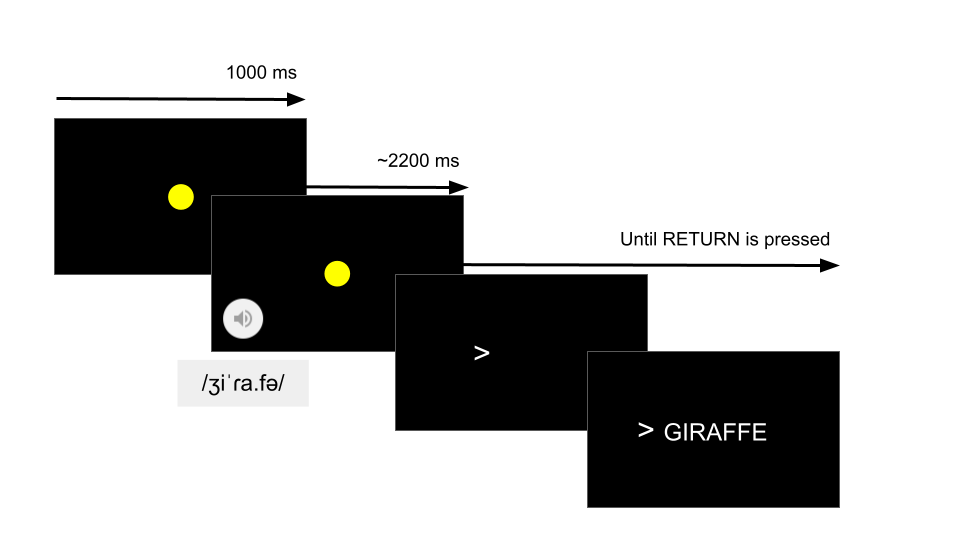
\includegraphics[width=0.8\linewidth]{C:/Users/u155880/Documents/translation-elicitation/img/design} \caption{Schematic representation of a trial in the experimental task.}\label{fig:procedurefigure}
\end{figure}

\hypertarget{stimuli}{%
\subsection{Stimuli}\label{stimuli}}

\hypertarget{input-stimuli-catalanspanish}{%
\subsubsection{Input stimuli (Catalan/Spanish)}\label{input-stimuli-catalanspanish}}

We arranged two lists of input words to be presented to participants in the auditory modality: one in Catalan (to be presented to English and Spanish natives) and one in Spanish (to be presented to English natives only). Words in the Catalan list were 5.01 phonemes long on average (\emph{SD} = 1.48, Range = 2-8). Words in the Spanish list were 5.50 phonemes long on average (\emph{SD} = 1.46, Range = 3-9). Participants listened to one audio file in each trial, each containing a single word presented in isolation. The audio files were the same ones used in child experiments conducted in the Laboratori de Recerca en Infància of Universitat Pompeu Fabra (Barcelona, Spain). These audio files were recorded by a proficient Catalan-Spanish female bilingual from the Metropolitan Area of Barcelona in a child-directed manner. Catalan and Spanish words were recorded at 44,100 Hz in separate files in the same session, and then de-noised using Audacity and normalised at peak intensity using Praat (Broersma \& Weenink, 2021). The average duration of the audio files was 1.20 (\emph{SD} = 0.18, Range = 0.78-1.58). The average duration of the Catalan audio files was 1.23 seconds (\emph{SD} = 0.19, Range = 0.80-1.58), and the average duration of the Spanish audio files was 1.16 seconds (\emph{SD} = 0.15, Range = 0.78-1.53).

\hypertarget{participant-responses-englishspanish}{%
\subsubsection{Participant responses (English/Spanish)}\label{participant-responses-englishspanish}}

Responses given by English participants for Catalan presented words were 5.14 characters long on average (\emph{SD} = 1.57, Range = 3-9), while their translations to Spani responses given by Spanish participants for Catalan words were 5.44 characters long on average (\emph{SD} = 1.56, Range = 3-9). Responses tgiven by English participants for Spanish words were 5.27 characters long on average (\emph{SD} = 1.75, Range = 3-12).

\hypertarget{target-translation-lexical-frequency}{%
\paragraph{Target translation lexical frequency}\label{target-translation-lexical-frequency}}

We extracted the lexical frequencies for English target translations from SUBTLEX-UK(Van Heuven et al., 2014), and frequencies for Spanish from SUBTLEX-ESP (Cuetos et al., 2011). We extracted scores as Zipf scores where available or transformed raw scores to Zipf scores to correct their logarithmic distribution, limiting their range roughly between 0 and 7, allowing an easier interpretation of further analyses (Van Heuven et al., 2014).

\hypertarget{target-translation-phonological-neighbourhood-density-pthn}{%
\paragraph{Target translation phonological neighbourhood density (PTHN)}\label{target-translation-phonological-neighbourhood-density-pthn}}

We retrieved PTHN scores (Phonological Total Higher-frequency Neighbourhood size) of the English and Spanish target translations from the CLEARPOND database (Marian et al., 2012). PTHN scores indicate the number of phonological neighbours with higher lexical frequency than the target translation, as indicated by its frequency score in the corresponding SUBTLEX database. CLEARPOND defines a phonological neighbour as a word whose phonological transcription in International Phonetic Alphabet (IPA) format (generated from eSPEAK, \url{http://espeak.sourceforge.net/}) differs from that of the target translation in only one addition, deletion, or substitution. PTHN scores in CLEARPOND measure have been calculated using corpora of similar size across language, allowing reliable cross-language comparisons.

\begin{figure}
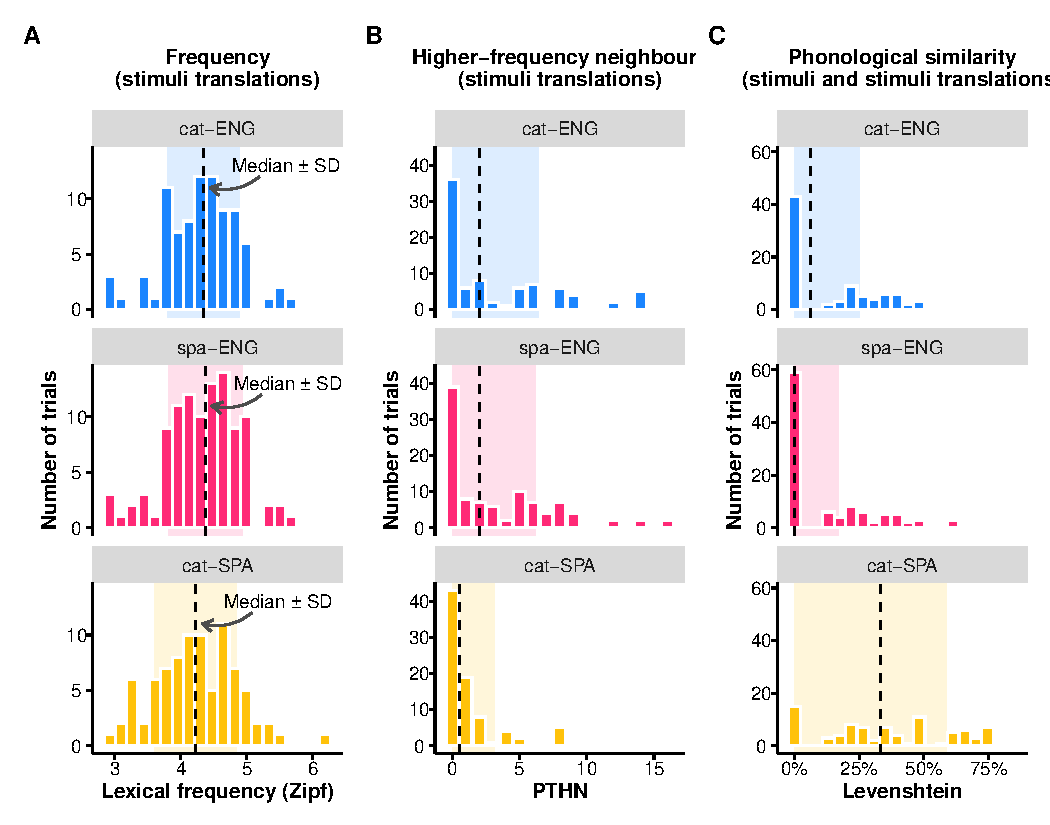
\includegraphics[width=1\linewidth]{manuscript_files/figure-latex/stimuliplot-1} \caption{Distribution and summary statistics of target translations, plotted in blue for English translations of Catalan stimuli (cat-ENG), pink for English translations of Spanish stimuli (spa-ENG), and yellow for Spanish translation of Catalan stimuli (cat-SPA). Columns indicate: A\) Lexical frequency of target translations, expressed as Zipf scores. B\) PTHN of target translations, and C\) Normalised Levenshtein phonological similarity between the presented words and their target translations, expressed in percentages. Lexical frequencies and PTHN scores of the presented words are not used in our analyses, as participants lack any lexical representation of such words.}\label{fig:stimuliplot}
\end{figure}

\hypertarget{cross-language-phonological-similarity-levenshtein}{%
\subsubsection{Cross-language phonological similarity (Levenshtein)}\label{cross-language-phonological-similarity-levenshtein}}

We measured the phonological similarity between presented words and their target translation by computing the Levenshtein similarity between their IPA transcriptions using the \texttt{stringsim} function of the stringdist R package (van der Loo, 2014). This function computes the inverse of the Levenshtein distance between two character strings as a proportion. First, it computes the edit distance between two character strings (in this case, phoneme transcriptions) by counting the number of additions, deletions, and substitutions necessary to make both strings identical (Levenshtein \& others, 1966). This measure is then divided by the maximum distance (according to the length of the longest string) and then subtracted from 1. The result is a percentage score, with 0\% indicating no similarity between the two strings, and 100\% indicating a perfect match between the two strings. We computed this similarity measure (refred simply as Levenshtein, from now on) for every translation pair in our stimuli lists. For example, the \emph{table} (\ipatext{'te<U+026A><U+0329>b<U+0259>l})-\emph{mesa} (mesa) translation pair had a 17\% similarity, while the \emph{train} (trEIn)-\emph{tren} (\ipatext{t<U+027E>en}) translation pair had a 60\% similarity. Figure 1 summarises the lexical frequency, phonological neighbourhood density and phonological overlap of the words included in the Catalan and the Spanish lists.

\hypertarget{data-analysis}{%
\subsection{Data analysis}\label{data-analysis}}

We modelled the probability of participants guessing the correct target translation of each presented word using a generalised multilevel Bayesian regression model with a Bernoulli logit link distribution. We first fitted a base model that only included the intercept as a fixed effect, and random intercepts per participant (Model 0). Secondly, we added the fixed effect of lexical frequency of the target translation (\(Frequency\)). We then extended the model sequentially by adding the main effect of higher-frequency phonological neighbourhood (\(PTHN\)), the main effect of Levenshtein similarity (\(Levenshtein\)), the \(PTHN \times Levenshtein\) interaction, the group of participants (\(Group\), with levels cat-ENG, spa-ENG, and cat-SPA), and finally, the \(Levenshtein \times Group\) interaction). We specified two sum-coded \emph{a priori} contrasts for the \(Group\) predictor: one comparing English natives (cat-ENG = -0.25, spa-ENG = -0.25) against Spanish natives (cat-SPA = +0.5), and one comparing English natives translating Spanish words (spa-ENG = -0.5) against English natives translating Catalan words (cat-ENG = +0.5) (Schad et al., 2020). Each model included random intercepts by item (to account for the correlation of responses from different participants to the same presented word), and random intercepts and slopes by participant, where our experimental designed allowed it (to account for the correlation between responses from the same participant to different presented words) (Barr et al., 2013). We will later refer to these models as Model 0 to Model 6. For interpretability, all continuous predictor variables were standardised (transformed in standard deviations from the mean) before entering the model.

\$\$\begin{align}

&\textbf{Likelihood}  \\
y_{i} \sim& Bernoulli(p_{i}) && \text{[probability of correct translation]} \\ \\

&\textbf{Parameters}  \\

logit(p_{i}) = ~ &  \beta_{0[p,w]} ~ +  && \text{[linear model]}\\
& \beta_{1[p]} ~ Frequency_{i} ~ + \\
& \beta_{2[p]} ~ PTHN_i ~ + \\
& \beta_{3[p]} ~ Similarity_i ~ + \\
& \beta_{4[p]} ~ (PTHN_i \times Similarity_i) \\ \\

\beta_{0-6[p,w]} \sim& ~  \mathcal{N}(\mu_{\beta_{j}}, \sigma_{\beta_{j}}) \text{, for participant } p ~\text{in 1, ..., } P ~\text{and  word } w ~\text{in 1, ..., } W && \text{[participant- and word-level intercepts]} \\
\beta_{1-6[p]} \sim& ~  \mathcal{N}(\mu_{\beta_{j}}, \sigma_{\beta_{j}}) \text{, for participant } p ~\text{in 1, ..., } P
&& \text{[participant-level coefficients]} \\ \\

&\textbf{Prior}  \\

\mu_{\beta_{p,w}} ~ \sim& ~ \mathcal{N}(0, 0.1) && \text{[participant-level coefficients]} \\
\sigma_{\beta_{p}}, ~ \sigma_{\beta_{w}} \sim& ~ HalfCauchy(0, 0.1) && \text{[SD for population and participant]} \\
\rho_{p}, ~ \rho_{w} \sim& ~LKJ(8) && \text{[correlation between participant-level coefficients]} \\


\end{align}\$\$

To test and account for cross-group differences, we included a random intercept for each group. We compared models using leave-one-out cross-validation (\emph{LOO}) (Vehtari et al., 2017). More information about the models and model comparison can be found in Appendix 2. All analyses were performed in R environment (RCore, 2019). We used the tidyverse family of R packages (Wickham et al., 2019) to process data and to generate figures. We used the brms R package (Bürkner, 2017) using the cmdstanr backend to the Stan probabilistic language (Carpenter et al., 2017) to estimate and compare the models (see Appendix 1 for mode details on the models).

\hypertarget{results}{%
\section{Results}\label{results}}

All models showed good out-of-sample predictive validity, as suggested by the fact that the expected log-probability density was many times larger than its associated standard error. Model 6, which included all main effects and the two-way interactions between \(PTHN\) and \(Levenshtein\), and between \(Group\) and \(Levenshtein\) and \(PTHN\) and consonant similarity, showed the best performance.

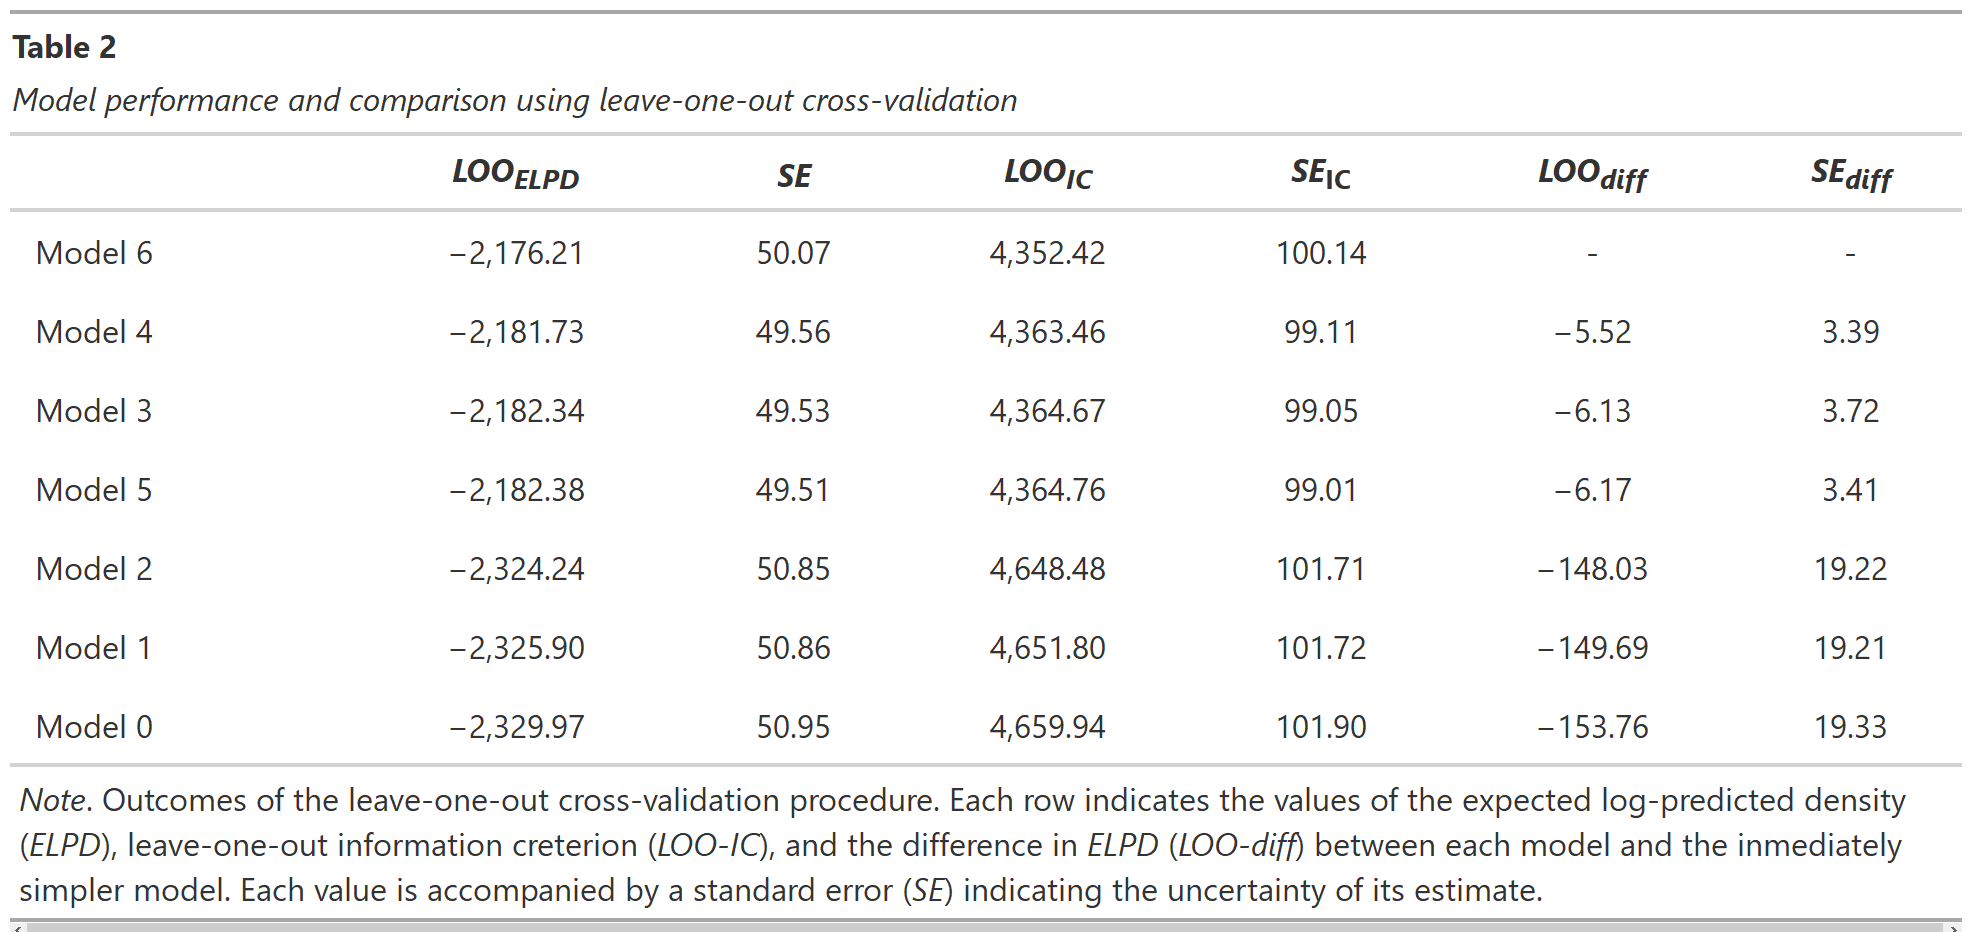
\includegraphics{C:/Users/u155880/Documents/translation-elicitation/img/loos.png}

We now report the mean of the posterior distribution of each coefficient in Model 6, along with its associated measures of uncertainty. For interpretability, we transformed the estimates of the intercept using the inverse logit function so that the values are expressed in probability of correct response instead of log-odds, and we transformed the coefficients of the rest of predictors divided by four. Dividing a coefficient expressed in log-odds by four returns an approximate of the derivative of the logistic function indicating the maximum steepness of the logistic curve. This way, the coefficients are expressed as increments or decrements in the probability of correct translation (Gelman et al., 2020).

\begin{figure}
\centering
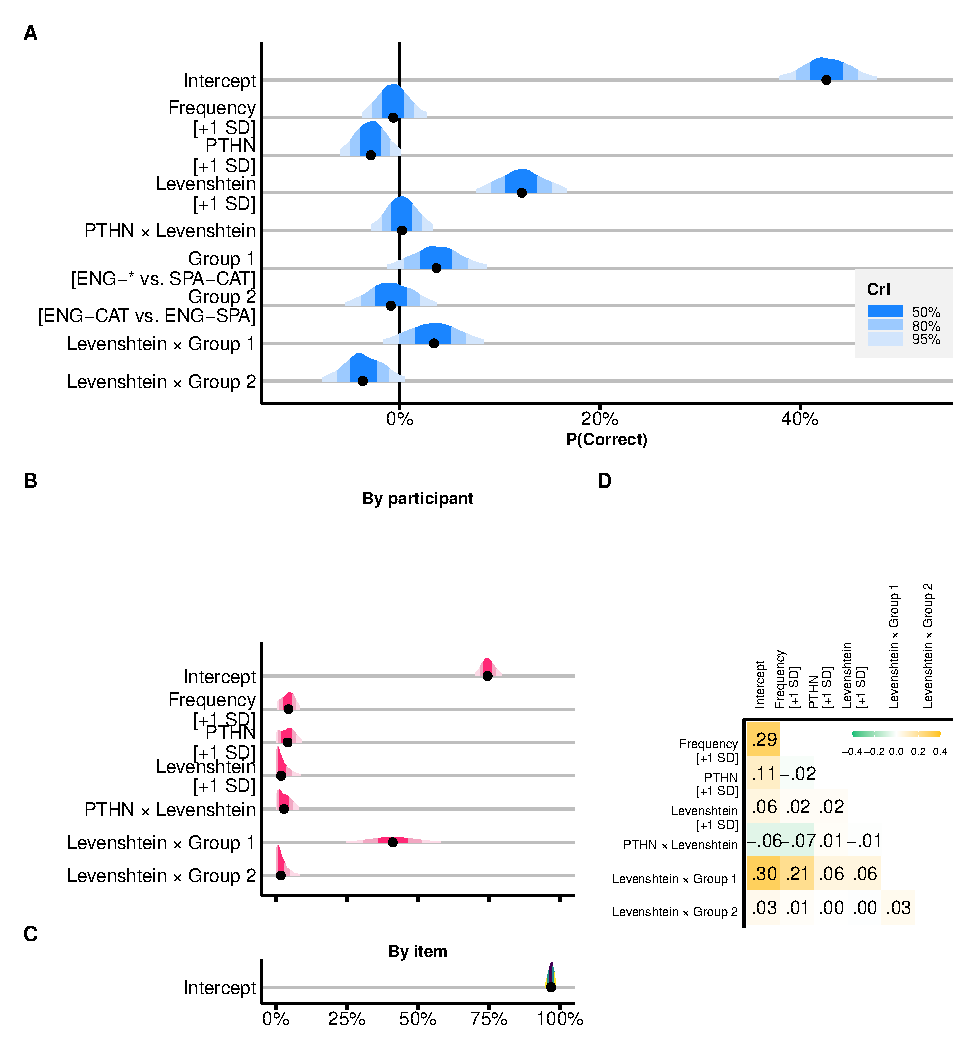
\includegraphics{manuscript_files/figure-latex/posteriorfix-1.pdf}
\caption{\label{fig:posteriorfix}Estimated posterior distributions of coefficients in Model 4. A) Population-level effects. Distributions indicate the estimated posterior likelihood density of regression coefficients of fixed effects. Credible intervals (\emph{CrI}), represented with increasingly lighter segmentents in the distribution indicate the range of values that contain the true value with 95\%, 80\%, and 50\% probability. Black dots represent the mean of each distribution. B) Participant-level coefficient variability. The model estimated participant-level coefficients to account for the dependency between responses from the same participant. Distributions in this panel indicate the estimated variability across coefficients from different participants, expressed as standard deviations (\emph{SD}). C) Correlation between participant-level effects. The model allowed participant-level coefficients to co-vary. This panel represents the Pearson correlations between each pair of coefficients, expressed as the mean of the posterior distribution of each estimated correlation.}
\end{figure}

Overall, participants had 43.08\%, (95\% \emph{CrI} = {[}38.20\%, 48.00\%{]}) likelihood to produce correct translations. The lexical frequency of the target translation had little impact on accuracy: every standard deviation increment (\emph{SD} = 0.57 Zipf points) decreased the probability of correct translation in 1.14\% (95\% \emph{CrI} = {[}1.14\%, -2.40\%{]}, \(BF_{\beta\neq< 0}\) = 1.20). The number of phonological neighbours with higher lexical frequency than the target translation (\emph{PTHN}) slightly decreased the probability of a correct responses by -1.70\% (95\% \emph{CrI} = {[}-5.26\%, 1.98\%{]}, \(BF_{\beta \neq 0}\) = 0.91) for every increase standard deviation increment (1 \emph{SD} = 3.94 neighbours). Finally, phonological similarity between the presented word and target translation had a strong effect on participants' accuracy: for every \emph{SD} increment in Levenshtein similarity (1 \emph{SD} = 23\% similarity), translation accuracy increased in 12.30\% (95\% \emph{CrI} = {[}7.48\%, 17.39\%{]}, \(BF_{\beta \neq 0}\) = \(>3.09 \times 10^{18}\)). The interaction effect between \(PTHN \times Levenshtein\) was small: a +1 SD increment in Levenshtein increased the effect of \emph{PTHN} by -0.11\% (95\% \emph{CrI} = {[}-3.72\%, 3.54\%{]}, \(BF_{\beta \neq 0}\) = 1.39)

Spanish natives translating Catalan words were 3.74\% more accurate than English natives translating Spanish and Catalan words (95\% \emph{CrI} = {[}-1.09\%, 8.64\%{]}, \(BF_{\beta \neq 0}\) = 0.35). The interaction between this contrast and Levenshtein suggests a moderate impact of phonological similarity on the difference between Spanish and English participants: this difference increased in 3.42\% for every one \emph{SD} increment in Levenshtein similarity (95\% \emph{CrI} = {[}-1.52\%, 8.45\%{]}, \(BF_{\beta \neq 0}\) = 0.41). English natives translating Catalan words were 0.60\% more accurate than those translating Spanish words (95\% \emph{CrI} = {[}-3.98\%, 5.17\%{]}, \(BF_{\beta \neq 0}\) = 1.00). For every one \emph{SD} increment in Levenshtein similarity, the effect of presented language increased in 3.08\% (95\% \emph{CrI} = {[}-1.24\%, 7.43\%{]}, \(BF_{\beta \neq 0}\) = 0.41).

\begin{figure}
\centering
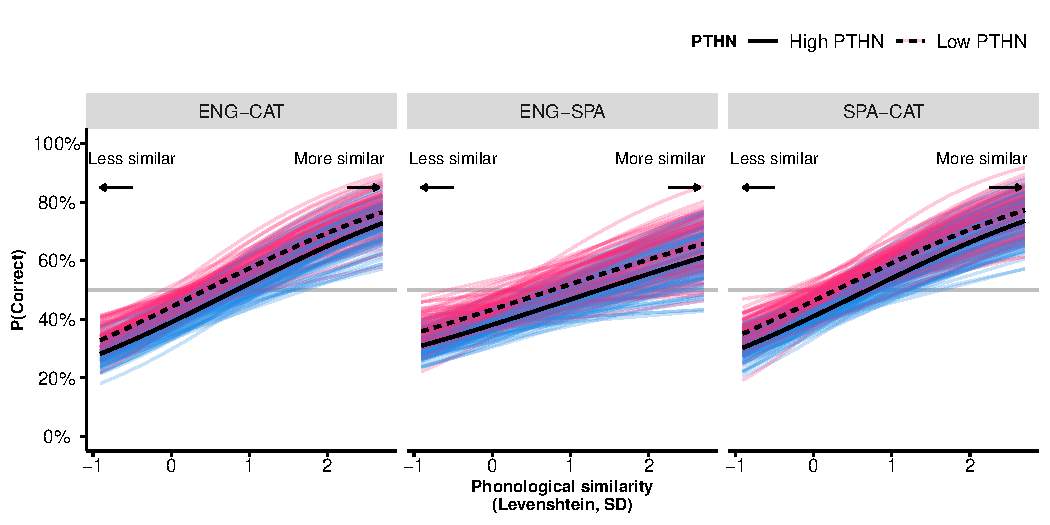
\includegraphics{manuscript_files/figure-latex/marginaleffects-1.pdf}
\caption{\label{fig:marginaleffects}Expected mean posterior predictions from Model 4. A) Population-level predictions: the X-axis and the Y-axis represent the PTHN score (in standard deviations from the mean) and the probability of correct translation, respectively. We simulated 300 observations from the posterior distribution of the model: 100 simulations for translations with no similarity (0\% Levenshtein), 100 simulations for translations with mean similarity (20.51\% Levenshtein), and 100 simulations for translations with the maximum similarity observed in the dataset (83.33\% Levenshtein). These simulations were obtained for the range of values of the PTHN scores. For each simulation, we drew a single sample from the posterior distribution of each coefficient. Each simulation is depicted in the graph as a line: pink for minimum similarity translations, blue for hight similarity translations, and yellow for maximum similarity translations. Black, thick lines indicate the expected mean value of the posterior predictions of the model for each condition. The dispersion of the lines indicates the uncertainty of our predictions. We computed these posterior predictions for each group of participants, and plot tem in separate panels.}
\end{figure}

The conditional intra-class correlation {[}\emph{ICC}; Gelman and Hill (2006){]} for items was 71.49\%, indicating that responses from different participants to the same item were, on average, more similar to each other than responses to other items. Item-level intercepts showed remarkable variability (\emph{SD} = 96.91\%, 95\% CrI = {[}94.66\%, 98.36\%{]}), indicating that participants' accuracy differed substantially across words: some words were very likely to be correctly translated (e.g., Spanish \emph{tomate}-\emph{tomato}, /tomate/-/təmɑːtoʊ/, 99.73\%, 95\% CrI = {[}96.40\%, 99.99\%{]}), while others were almost never translated correctly (e.g., Catalan \emph{colom}-\emph{pigeon}, /kulom/-/pɪdʒɪn/, 0.08\%, 95\% CrI = {[}0.00\%, 1.00\%{]}). Participant-level intercepts also showed high variability (\emph{SD} = 75.73\%, 95\% CrI = {[}71.33\%, 80.33\%{]}), suggesting that average translation accuracy also varied significantly across participants. Finally, participant-level estimated slopes showed less variability: \emph{SD} of \(Frequency\), \(PTHN\), \(Levenshtein\), \(PTHN \times Levenshtein\), and \(Levenshtein \times Group 2\) ranged between 2.56\%, and 37.19\%. The participant-level estimated slopes of the \(Leveshtein \times Group 1\) interaction are an exception, though (\emph{SD} = 37.19\%, 95\% CrI = {[}14.92\%, {]}). This indicates that the impact of phonological similarity (\(Levenshtein\)) on the difference in accuracy between English and Spanish natives differed substantially across participants.

Finally, participant-level effects showed weak Pearson correlations overall (\textless10\%), with three exceptions. The estimated correlation between the intercepts and the slopes of \(Frequency\) was 35.81\% (95\% CrI = {[}-2.19\%, 65.22\%{]}, \(BF_{Cor \neq 0}\) = 0.15). The estimated correlation between the slopes of \(Frequency\) and \(Levenshtein \times Group 1\) was 26.07\% (95\% CrI = {[}-13.12\%, 57.14\%{]}, \(BF_{Cor \neq 0}\) = 0.37). The estimated correlation between the intercepts and the slopes of \(PTHN\) was 1.81\% (95\% CrI = {[}-39.01\%, 38.35\%{]}, \(BF_{Cor \neq 0}\) = 1). The large uncertainty associated with these estimates, however, prevents us from interpreting the size of these correlations as practically meaningful.

\hypertarget{discussion}{%
\section{Discussion}\label{discussion}}

\newpage

\hypertarget{references}{%
\section{References}\label{references}}

\begingroup
\setlength{\parindent}{-0.5in}
\setlength{\leftskip}{0.5in}

\hypertarget{refs}{}
\begin{CSLReferences}{1}{0}
\leavevmode\vadjust pre{\hypertarget{ref-barr2013random}{}}%
Barr, D. J., Levy, R., Scheepers, C., \& Tily, H. J. (2013). Random effects structure for confirmatory hypothesis testing: Keep it maximal. \emph{Journal of Memory and Language}, \emph{68}(3), 255--278.

\leavevmode\vadjust pre{\hypertarget{ref-best2001discrimination}{}}%
Best, C. T., McRoberts, G. W., \& Goodell, E. (2001). Discrimination of non-native consonant contrasts varying in perceptual assimilation to the listener's native phonological system. \emph{The Journal of the Acoustical Society of America}, \emph{109}(2), 775--794.

\leavevmode\vadjust pre{\hypertarget{ref-broersma2021praat}{}}%
Broersma, P., \& Weenink, D. (2021). \emph{Praat: Doing phonetics by computer {[}computer program{]}} (Version 6.1.54). \url{http://www.praat.org/}

\leavevmode\vadjust pre{\hypertarget{ref-burkner2017brms}{}}%
Bürkner, P.-C. (2017). Brms: An r package for bayesian multilevel models using stan. \emph{Journal of Statistical Software}, \emph{80}(1), 1--28.

\leavevmode\vadjust pre{\hypertarget{ref-carpenter2017stan}{}}%
Carpenter, B., Gelman, A., Hoffman, M. D., Lee, D., Goodrich, B., Betancourt, M., Brubaker, M. A., Guo, J., Li, P., \& Riddell, A. (2017). Stan: A probabilistic programming language. \emph{Grantee Submission}, \emph{76}(1), 1--32.

\leavevmode\vadjust pre{\hypertarget{ref-chen1989patterns}{}}%
Chen, H.-C., \& Leung, Y.-S. (1989). Patterns of lexical processing in a nonnative language. \emph{Journal of Experimental Psychology: Learning, Memory, and Cognition}, \emph{15}(2), 316.

\leavevmode\vadjust pre{\hypertarget{ref-christoffels2006memory}{}}%
Christoffels, I. K., De Groot, A. M., \& Kroll, J. F. (2006). Memory and language skills in simultaneous interpreters: The role of expertise and language proficiency. \emph{Journal of Memory and Language}, \emph{54}(3), 324--345.

\leavevmode\vadjust pre{\hypertarget{ref-christoffels2013language}{}}%
Christoffels, I. K., Ganushchak, L., \& Koester, D. (2013). Language conflict in translation: An ERP study of translation production. \emph{Journal of Cognitive Psychology}, \emph{25}(5), 646--664.

\leavevmode\vadjust pre{\hypertarget{ref-costa2000cognate}{}}%
Costa, A., Caramazza, A., \& Sebastian-Galles, N. (2000). The cognate facilitation effect: Implications for models of lexical access. \emph{Journal of Experimental Psychology: Learning, Memory, and Cognition}, \emph{26}(5), 1283.

\leavevmode\vadjust pre{\hypertarget{ref-cuetos2011subtlex}{}}%
Cuetos, F., Glez-Nosti, M., Barbon, A., \& Brysbaert, M. (2011). SUBTLEX-ESP: Frecuencias de las palabras espanolas basadas en los subtitulos de las peliculas. \emph{Psicol{ó}gica}, \emph{32}(2), 133--144.

\leavevmode\vadjust pre{\hypertarget{ref-cutler2004patterns}{}}%
Cutler, A., Weber, A., Smits, R., \& Cooper, N. (2004). Patterns of english phoneme confusions by native and non-native listeners. \emph{The Journal of the Acoustical Society of America}, \emph{116}(6), 3668--3678.

\leavevmode\vadjust pre{\hypertarget{ref-de2000hard}{}}%
De Groot, A. M., \& Keijzer, R. (2000). What is hard to learn is easy to forget: The roles of word concreteness, cognate status, and word frequency in foreign-language vocabulary learning and forgetting. \emph{Language Learning}, \emph{50}(1), 1--56.

\leavevmode\vadjust pre{\hypertarget{ref-dijkstra2002architecture}{}}%
Dijkstra, T., \& Van Heuven, W. J. (2002). The architecture of the bilingual word recognition system: From identification to decision. \emph{Bilingualism: Language and Cognition}, \emph{5}(3), 175--197.

\leavevmode\vadjust pre{\hypertarget{ref-dijkstra2019multilink}{}}%
Dijkstra, T., Wahl, A., Buytenhuijs, F., Van Halem, N., Al-Jibouri, Z., De Korte, M., \& Rekké, S. (2019). Multilink: A computational model for bilingual word recognition and word translation. \emph{Bilingualism: Language and Cognition}, \emph{22}(4), 657--679.

\leavevmode\vadjust pre{\hypertarget{ref-elias2022cross}{}}%
Elias, M., \& Degani, T. (2022). Cross-language interactions during novel word learning: The contribution of form similarity and participant characteristics. \emph{Bilingualism: Language and Cognition}, 1--18.

\leavevmode\vadjust pre{\hypertarget{ref-floccia2018introduction}{}}%
Floccia, C., Sambrook, T. D., Delle Luche, C., Kwok, R., Goslin, J., White, L., Cattani, A., Sullivan, E., Abbot-Smith, K., Krott, A., \& others. (2018). I: INTRODUCTION. \emph{Monographs of the Society for Research in Child Development}, \emph{83}(1), 7--29.

\leavevmode\vadjust pre{\hypertarget{ref-gelman2006data}{}}%
Gelman, A., \& Hill, J. (2006). \emph{Data analysis using regression and multilevel/hierarchical models}. Cambridge university press.

\leavevmode\vadjust pre{\hypertarget{ref-gelman2020regression}{}}%
Gelman, A., Hill, J., \& Vehtari, A. (2020). \emph{Regression and other stories}. Cambridge University Press.

\leavevmode\vadjust pre{\hypertarget{ref-goldinger1989priming}{}}%
Goldinger, S. D., Luce, P. A., \& Pisoni, D. B. (1989). Priming lexical neighbors of spoken words: Effects of competition and inhibition. \emph{Journal of Memory and Language}, \emph{28}(5), 501--518.

\leavevmode\vadjust pre{\hypertarget{ref-gooskens2004perceptive}{}}%
Gooskens, C., \& Heeringa, W. (2004). Perceptive evaluation of levenshtein dialect distance measurements using norwegian dialect data. \emph{Language Variation and Change}, \emph{16}(3), 189--207.

\leavevmode\vadjust pre{\hypertarget{ref-de1992determinants}{}}%
Groot, A. M. de. (1992). Determinants of word translation. \emph{Journal of Experimental Psychology: Learning, Memory, and Cognition}, \emph{18}(5), 1001.

\leavevmode\vadjust pre{\hypertarget{ref-degroot1994forward}{}}%
Groot, A. M. de, Dannenburg, L., \& Vanhell, J. G. (1994). Forward and backward word translation by bilinguals. \emph{Journal of Memory and Language}, \emph{33}(5), 600--629.

\leavevmode\vadjust pre{\hypertarget{ref-kroll1994category}{}}%
Kroll, J. F., \& Stewart, E. (1994). Category interference in translation and picture naming: Evidence for asymmetric connections between bilingual memory representations. \emph{Journal of Memory and Language}, \emph{33}(2), 149--174.

\leavevmode\vadjust pre{\hypertarget{ref-lecumberri2010non}{}}%
Lecumberri, M. L. G., Cooke, M., \& Cutler, A. (2010). Non-native speech perception in adverse conditions: A review. \emph{Speech Communication}, \emph{52}(11-12), 864--886.

\leavevmode\vadjust pre{\hypertarget{ref-levenshtein1966binary}{}}%
Levenshtein, V. I., \& others. (1966). Binary codes capable of correcting deletions, insertions, and reversals. \emph{Soviet Physics Doklady}, \emph{10}, 707--710.

\leavevmode\vadjust pre{\hypertarget{ref-lotto1998effects}{}}%
Lotto, L., \& De Groot, A. M. (1998). Effects of learning method and word type on acquiring vocabulary in an unfamiliar language. \emph{Language Learning}, \emph{48}(1), 31--69.

\leavevmode\vadjust pre{\hypertarget{ref-luce1998recognizing}{}}%
Luce, P. A., \& Pisoni, D. B. (1998). Recognizing spoken words: The neighborhood activation model. \emph{Ear and Hearing}, \emph{19}(1), 1.

\leavevmode\vadjust pre{\hypertarget{ref-luce1990similarity}{}}%
Luce, P. A., Pisoni, D. B., \& Goldinger, S. D. (1990). \emph{Similarity neighborhoods of spoken words.}

\leavevmode\vadjust pre{\hypertarget{ref-marian2012clearpond}{}}%
Marian, V., Bartolotti, J., Chabal, S., \& Shook, A. (2012). \emph{CLEARPOND: Cross-linguistic easy-access resource for phonological and orthographic neighborhood densities}.

\leavevmode\vadjust pre{\hypertarget{ref-mcclelland1981interactive}{}}%
McClelland, J. L., \& Rumelhart, D. E. (1981). An interactive activation model of context effects in letter perception: I. An account of basic findings. \emph{Psychological Review}, \emph{88}(5), 375.

\leavevmode\vadjust pre{\hypertarget{ref-midgley2011effects}{}}%
Midgley, K. J., Holcomb, P. J., \& Grainger, J. (2011). Effects of cognate status on word comprehension in second language learners: An ERP investigation. \emph{Journal of Cognitive Neuroscience}, \emph{23}(7), 1634--1647.

\leavevmode\vadjust pre{\hypertarget{ref-peirce2019psychopy2}{}}%
Peirce, J., Gray, J. R., Simpson, S., MacAskill, M., Höchenberger, R., Sogo, H., Kastman, E., \& Lindeløv, J. K. (2019). PsychoPy2: Experiments in behavior made easy. \emph{Behavior Research Methods}, \emph{51}(1), 195--203.

\leavevmode\vadjust pre{\hypertarget{ref-potter1984lexical}{}}%
Potter, M. C., So, K.-F., Von Eckardt, B., \& Feldman, L. B. (1984). Lexical and conceptual representation in beginning and proficient bilinguals. \emph{Journal of Verbal Learning and Verbal Behavior}, \emph{23}(1), 23--38.

\leavevmode\vadjust pre{\hypertarget{ref-rcore2019r}{}}%
RCore, T. (2019). \emph{R: A language and environment for statistical computing. R foundation for statistical computing, austria}.

\leavevmode\vadjust pre{\hypertarget{ref-schad2020capitalize}{}}%
Schad, D. J., Vasishth, S., Hohenstein, S., \& Kliegl, R. (2020). How to capitalize on a priori contrasts in linear (mixed) models: A tutorial. \emph{Journal of Memory and Language}, \emph{110}, 104038.

\leavevmode\vadjust pre{\hypertarget{ref-schepens2012distributions}{}}%
Schepens, J., Dijkstra, T., \& Grootjen, F. (2012). Distributions of cognates in europe as based on levenshtein distance. \emph{Bilingualism: Language and Cognition}, \emph{15}(1), 157--166.

\leavevmode\vadjust pre{\hypertarget{ref-takata1990english}{}}%
Takata, Y., \& Nábělek, A. K. (1990). English consonant recognition in noise and in reverberation by japanese and american listeners. \emph{The Journal of the Acoustical Society of America}, \emph{88}(2), 663--666.

\leavevmode\vadjust pre{\hypertarget{ref-thierry2007brain}{}}%
Thierry, G., \& Wu, Y. J. (2007). Brain potentials reveal unconscious translation during foreign-language comprehension. \emph{Proceedings of the National Academy of Sciences}, \emph{104}(30), 12530--12535.

\leavevmode\vadjust pre{\hypertarget{ref-valente2018does}{}}%
Valente, D., Ferré, P., Soares, A., Rato, A., \& Comesaña, M. (2018). Does phonological overlap of cognate words modulate cognate acquisition and processing in developing and skilled readers? \emph{Language Acquisition}, \emph{25}(4), 438--453.

\leavevmode\vadjust pre{\hypertarget{ref-van2014stringdist}{}}%
van der Loo, M. P. J. (2014). The stringdist package for approximate string matching. \emph{The {R} {J}ournal}, \emph{6}, 111--122. \url{https://CRAN.R-project.org/package=stringdist}

\leavevmode\vadjust pre{\hypertarget{ref-van1998orthographic}{}}%
Van Heuven, W. J., Dijkstra, T., \& Grainger, J. (1998). Orthographic neighborhood effects in bilingual word recognition. \emph{Journal of Memory and Language}, \emph{39}(3), 458--483.

\leavevmode\vadjust pre{\hypertarget{ref-van2014subtlex}{}}%
Van Heuven, W. J., Mandera, P., Keuleers, E., \& Brysbaert, M. (2014). SUBTLEX-UK: A new and improved word frequency database for british english. \emph{Quarterly Journal of Experimental Psychology}, \emph{67}(6), 1176--1190.

\leavevmode\vadjust pre{\hypertarget{ref-vehtari2017practical}{}}%
Vehtari, A., Gelman, A., \& Gabry, J. (2017). Practical bayesian model evaluation using leave-one-out cross-validation and WAIC. \emph{Statistics and Computing}, \emph{27}(5), 1413--1432.

\leavevmode\vadjust pre{\hypertarget{ref-weber2004lexical}{}}%
Weber, A., \& Cutler, A. (2004). Lexical competition in non-native spoken-word recognition. \emph{Journal of Memory and Language}, \emph{50}(1), 1--25.

\leavevmode\vadjust pre{\hypertarget{ref-wickham2019tidyverse}{}}%
Wickham, H., Averick, M., Bryan, J., Chang, W., McGowan, L. D., François, R., Grolemund, G., Hayes, A., Henry, L., Hester, J., Kuhn, M., Pedersen, T. L., Miller, E., Bache, S. M., Müller, K., Ooms, J., Robinson, D., Seidel, D. P., Spinu, V., \ldots{} Yutani, H. (2019). Welcome to the {tidyverse}. \emph{Journal of Open Source Software}, \emph{4}(43), 1686. \url{https://doi.org/10.21105/joss.01686}

\end{CSLReferences}

\endgroup

\newpage


\end{document}
